\documentclass[
  journal=bjps
]{cup-journal}

% Packages for the example
\usepackage{booktabs,microtype,siunitx,tabularx}
\usepackage{graphicx} % Graphics
\usepackage{indentfirst} % Tells LaTeX to indent every paragraph 
\usepackage{setspace} % To set line spacing
\usepackage{rotating} % For sideways tables/figures
\usepackage{amsmath} % Some math symbols
\usepackage{subfig}
\usepackage{mdwlist}
\usepackage{url}
\usepackage{verbatim}
\urlstyle{same}
\usepackage{multirow}
%\usepackage[nolists]{endfloat} % Figures and tables at the end
\newcommand{\R}{\texttt{R}\space} % Write R in typewriter font
\newcommand{\trans}[1]{{#1}^{\ensuremath{\mathsf{T}}}} % Transpose symbol 
\sisetup{detect-all,separate-uncertainty = true}

\addbibresource{sources.bib}

\title{How ``Rage Bait'' and Outgroup Cues Strengthen Support for Violence and Anti-Muslim Policies}

%\author{Jeffrey\ Javed}
%\affiliation{Former Research Fellow, Weiser Center for Emerging Democracies, University of Michigan}
%\author{Blake\ Miller}
%\affiliation{Assistant Professor, London School of Economics}
%\email{b.a.miller@lse.ac.uk}

%\doi{10.1017/S0007123421000132}

%\received {}
%\revised  {}
%\accepted {}
%\published{}

\keywords{hate speech; political violence; content moderation}
% \jel{Q11; Q12; D81; M31}
% \msc{Q14; Q18; E21}
% \abbreviations{
%     BDHS: Bangladesh Demographic and Health Survey, 
%     IDA: Fe-deficiency anaemia, 
%     IFA: Fe-folic acid, 
%     MNP: multiple micronutrient powder, 
%     VAD: vitamin A deficiency
% }

\begin{document}

\begin{abstract}
\noindent Existing research has acknowledged online information as a source of violent and discriminatory behavior. However, this research has primarily focused on its diffusion rather than its substantive effects. This study examines what kind of information drives violence and discrimination, testing the effects of sensationalization, outgroup cues, and public opinion perception on support for violence and anti-Muslim policies. We test this with an online survey experiment via a realistic, interactive website treatment detailing a homicide story in small-town America. We find that sensational language increased individuals' support for violence by provoking feelings of anger and fear. Further, we found that identifying the suspect in the homicide as a Muslim refugee, versus specifying no outgroup affiliation, increased support for anti-Muslim policies. Lastly, perceived public support for violence increased the likelihood of upvoting or writing violent comments. This study contributes to our understanding of the effects of sensational news and public debate on online content moderation.
\end{abstract}

\section{Introduction}

An important yet under-examined subset of misinformation is popularly known as ``rage bait'' or ``outrage bait'': highly sensationalized content that intentionally enrages the reader through selective reporting or false information. This type of misinformation uses emotionally and morally charged language to solicit this outrage. Rage bait has become particularly dominant online. People are more likely to encounter content that induces outrage online \citep{crockett2017moral}, and content rich in moral-emotional language is more likely to go viral \citep{brady2017emotion, fan2014anger}. Alarmingly, people report much higher levels of outrage when encountering this kind of content on social media than in-person or on traditional forms of media like TV and radio \citep{crockett2017moral}.

Rage-bait can come in many forms: news or news-like articles, social media posts, TikTok videos, etc. It is sometimes original content, but is often ``stitched'' or refactored content from another producer. One example of a rage bait article is the article that incited the ``Pizzagate'' incident (see Figure \ref{fig:example}). The article styled itself as an investigative news report, lending credence to false rumors that Anthony Wiener's leaked emails had revealed a pedophilia ring linked to the Clintons in the Comet Ping Pong pizzeria in Washington, D.C. After the article's publication, many were mobilized to harrass employees and the owners, including an individual who discharged his gun in the pizzeria in an attempt to save children he thought were being abused in the (nonexistent) basement. Another example is the ``Libs of TikTok'' Twitter/X account which grew in popularity in 2020 by reposting TikTok videos of LGBTQ+ professionals working in child-facing roles (e.g., bus drivers, nurses, teachers, etc.). Commentary on reposted videos often primes followers with the unsubstantiated moral panic about LGBTQ+ people ``grooming'' children (see Figure \ref{fig:example}). Many of the individuals featured on this account have experienced death threats. Additionally, two children's hospitals and eleven schools have received bomb threats after the account owner Chaya Raichik made posts about their employees \citep{yang2022boston, lorenz2022lgbt, anguiano2023california}.

\begin{figure}[h]
  \centering
  \caption{Examples of Rage-Bait}
  \includegraphics[width=\textwidth]{figures/rage_bait_examples.png}
  \label{fig:example}
  {\footnotesize Left: The false news article that (falsely) substantiated Pizzagate rumors; Right: A post by Libs of Tiktok implying LGBT grooming of children. Both articles resulted in violence.}
\end{figure}

While rage bait has received scant academic attention, social media platforms have created extensive tools and policies to regulate the distribution of sensationalized content and other forms of ``inauthentic'' content. Facebook's News Feed policy, emphasizing its commitment to ``authentic communication,'' enforces against posts that ``[e]xaggerate or sensationalize content in a headline and mislead readers'' and warns of sanctions against Facebook Pages and domains that consistently purvey such content \citep{facebook2021}. Twitter's general terms of use policy, under the heading of ``Authenticity,'' forbids users from using the platform ``to artificially amplify or suppress information or engage in behavior that manipulates or disrupts people’s experience on Twitter.'' \citep{twitter2021}. Similarly, Youtube's Community Guidelines forbid ``deceptive practices that take advantage of the YouTube community'' \citep{youtube2021}.

These social media platform policies exist alongside extensive media coverage that has frequently linked the dissemination of ``rage bait''-like stories---particularly those detailing sensationalized accounts of criminality or moral wrongdoing---to politically-motivated attempts to mobilize violence against vulnerable minority groups. For example, in India, the largest market for Facebook's WhatsApp platform, political parties have used WhatsApp to spread false and sensationalized stories of murder and religious sacrilege by Muslims to inflame Muslim-Hindu tensions \citep{parth2018}. A United Nations report claimed that the military in Myanmar had disseminated sensational, false news on Facebook that may have driven genocidal violence against the Rohingya \citep{mozur2018}. Non-state actors similarly use sensationalized and false news toward violent ends. The Sri Lankan government blocked Facebook after witnessing an increase in mob violence in response to fake, sensationalized content about the alleged misdeeds of Muslims spread by extremist groups \citep{goel2018b}. Rage bait has a long history in the United States. White Americans have historically targeted thousands of Black Americans with extrajudicial violence, including racial-political killings. In many cases, they mobilized violence through sensationalized news reporting of alleged moral transgressions of Black Americans \citep{francis2020white}. In recent years, the proliferation of sensational anti-immigrant news from the American alt-right has coincided with a dramatic rise in the number of reported hate crimes, as recorded by the FBI and the Southern Poverty Law Center \citep{barrett_2018}. While systematic data on American alt-right content creators' intent are unavailable, there is anecdotal evidence that some of these producers intentionally seek to promote or normalize violence. Notably, a leaked ``style manual'' from the neo-Nazi website \textit{The Daily Stormer} instructed its writers: ``It's illegal to promote violence on the Internet. At the same time, it’s totally important to normalize the acceptance of violence as an eventuality/inevitability'' \citep{feinberg2017daily}. 

Under what conditions does rage bait--news stories featuring sensationalized claims of wrongdoings--affect mass attitudes toward the acceptability of violence? Despite growing concerns over the global proliferation of misinformation through social media, we know more about its patterns of diffusion than its effects \citep{brady2017emotion, lazer2018fakenews, vosoughi2018spread}; and we know nearly nothing about its effects on violent attitudes and behavior. Social media provides strong economic incentives to produce and spread sensationalized, outrage-inducing content \citep{crockett2017moral}. However, we do not know if sensational content increases the acceptability of violence, nor do we understand the cognitive mechanisms by which such an effect would occur. Research on related phenomena of hate speech and propaganda provide scant guidance: research has focused mainly on the legal and ethical dimensions of hate speech moderation and less on its real-world effects \citep{gates1996speaking,waldron2012harm}, and observational research on genocidal propaganda has produced mixed results \citep{fujii2004transforming, hagan2008darfur,  straus2007relationship,yanagizawa2014propaganda}. While some scholars have found links between the consumption of violent media and aggressive behavior \citep{kalmoe2014fueling}, most of these findings are limited in scope to children \citep{anderson2003dissociating,drabman1974does,huesmann1994long}. 

Our study examines the effects of sensationalization, outgroup cues, and public opinion perception on support for violence and anti-Muslim policies. We used an online 2$^3$ factorial experiment with a realistic, interactive website treatment detailing a homicide story in small-town America, written in the style of a sensationalized, anti-immigrant news article that routinely appear on alt-right news platforms. Through an analysis of open-ended survey text, and online behavioral data, we find that sensational content---which we define as text, images, and videos that employ moral-emotional language\footnote{Moral emotions are feelings relating to ``evaluations of societal norms'' \citep{brady2017emotion}, specifically ``feelings that stem from violating evaluative cultural codes, that is, codes that indicate what is good or bad or right or wrong in a society'' \citep{stets2012current}. To understand moral-emotional language, we draw on \citep{brady2017emotion}'s dictionary of moral-emotional language, which contains words in the overlap between previously validated dictionaries of moral language and emotional language from the Linguistic Inquiry and Word Count (LIWC).} to present claims of moral violation or wrongdoing---increases individuals' endorsement of violence by provoking anger and fear. Also, we find that identifying the suspect in the homicide as a Muslim refugee, versus specifying no outgroup affiliation, increased support for anti-Muslim policies, while perceived public support for violence increased the likelihood of upvoting or writing violent comments. 

This argument builds on research in social psychology that suggests that exposure to moral violations lowers an individual's threshold for using violence against perceived norm violators by provoking outrage and providing justifications for their punishment \citep{baumeister1999evil,beck1999prisoners,crockett2017moral, fiske2014virtuous, goldberg1999rage} and explores the mechanisms by which political and non-state actors can mobilize a critical mass of support for violence among the public. The rest of this article proceeds as follows. The next section briefly reviews the literature on political violence, political mobilization, and emotion. We then detail our experimental design and variable measurement strategies and present our results. The final section concludes with a discussion of how these findings apply to rage-bait, the false news phenomenon, and violent political mobilization more generally.

\section{Literature}

\begin{comment}
    - kalmoe2022radical: "links."
    - cassese2019reconciling - Cassese 2019, Political Behavior
    - vasilopoulos2019fear: Vasilopoulos, Marcus, and Valentino similar findings but with a more explicit theory. "support for authoritarian policies against terrorism"
\end{comment}

Rage bait lies on the spectrum of misinformation. While rage bait content may not be completely false, it relies on moral and emotional content to activate anger and fear, emotions associated with virality of content on social networks such as Twitter \citep{brady2017emotion}. It is related to but distinct from clickbait, which Benkler et al. (2018, p. 9) define as ``media items designed to trigger an affective response from a user that leads them to click on the item...because the click itself generates revenue from the clickbait purveyor.'' While there are clear monetary incentives for media outlets to publish rage bait, purveyors of rage bait are not necessarily motivated by revenue alone. The QAnon conspiracy movement disseminated an abundance of rage bait alleging establishment politicians were Satan-worshipping pedophiles in order to spread their beliefs and attract new converts. 

The use of sensationalized content to foment violence against vulnerable populations is nothing new: the scholarship on collective violence, genocide, and war has long noted the outsized role of fabricated, sensational content in promoting violence against a targeted outgroup \citep{charny2019can, cohn1967warrant, dower1986war, fein1979accounting, herf2006jewish, hill1995delusion, goldhagen1997hitler, goldhagen2009worse, tsesis2002destructive}. For example, the circulation of Cotton Mather's \textit{Memorable Providences} detailing ``real'' accounts of bewitchings of innocent children is thought to have fueled the persecution of ``witches'' in the Massachusetts Bay Colony \citep{hill1995delusion}; the \textit{Protocols of the Elders of Zion}, which described a plan for Jewish world domination, was an important precursor to anti-Semitic Nazi mobilization \citep{cohn1967warrant,herf2006jewish}; and sensationalized accounts of Japanese atrocities against American POWs featured heavily in American anti-Japanese propaganda designed to recruit soldiers and bolster their fighting spirit \citep{dower1986war}. 

Few scholars, however, have directly tested the causal effects of content on violent attitudes, and the results of these studies have been mixed. Looking at political attitudes, \cite{kalmoe2014fueling} finds that violent rhetoric interacts with trait aggression to increase support for partisan political violence. \cite{kalmoe2022radical} find that partisan dehumanization and out-group vilification increase support for partisan violence. In the context of genocidal violence, \cite{hagan2008darfur} find that the use of dehumanizing racial epithets during attacks on black African populations in Darfur correlated with more extreme violence. Other scholars have challenged the causal link between hateful content and violence. Looking at the Rwandan genocide, \cite{straus2007relationship} argues that the spatial coverage of Hutu-controlled ``hate radio'' cannot explain the geographic variation in the onset of violence, while others have argued that anti-Tutsi propaganda was critical to driving violence or, at the very least, normalizing it \citep{fujii2004transforming, yanagizawa2014propaganda}.

Moreover, it is unclear what kinds of content promote violence. Though scholars have emphasized the primacy of dehumanizing content in genocidal violence \citep{fein1979accounting, charny1982can}, there is little empirical evidence for its efficacy. A major underexplored alternative is moral frameworks that justify the righteousness of violence \citep{viterna2014radical, javed2022righteous}. Social psychologists have long emphasized the significance of morality---conceptions of right and wrong traits and behaviors---in understanding participation in violence, private and political \citep{bandura1975disinhibition,baumeister1999evil,beck1999prisoners,fiske2014virtuous}. Because using violence requires first overcoming formidable moral-emotional reservations, moral narratives that condone and justify violence can erode these otherwise powerful restraints on violent behavior \citep{baumeister1999evil,beck1999prisoners,fincher2016perceptual}. Moralistic content may also mobilize participation in violent causes by drawing upon individuals' latent moral convictions. \cite{wood2003insurgent} emphasizes the pleasure of agency that participants derive from acting on their moral convictions in a movement, which \cite{viterna2014radical} extends to the willingness of citizens to accept violence in the name of righteous causes, movements where ``interested publics believe that the enactors of political violence are defending society's most vulnerable and protecting a morally legitimate social order.'' Indeed, \cite{kirkpatrick2008uncivil} documents a long history of extrajudicial and vigilante violence in America that invokes revolutionary values of freedom, justice, and democracy to frame itself as righteous.

In addition to appeals to morality, it is clear that appeals to---and activation of---negative emotions serve an important role in the mobilization of violence. The political ramifications of negative emotions have been widely studied, particularly in the context of political behavior and attitudes following terrorist attacks. Studies in this area reveal that the intensity of emotions, specifically fear and anger, leads to the emergence of markedly different attitudes. \cite{lerner2003effects} discovered that fear prompted more optimistic risk assessments post-attacks, while anger contributed to a more pessimistic outlook. Further research by \cite{huddy2011americans} and \cite{skitka2006confrontational} links post-9/11 anger towards terrorists to the endorsement of strong governmental or military responses. \cite{vasilopoulos2019fear}, whose work---also examining attitudes in the wake of a terror attack---suggests that public support for far-right politics is more likely rooted in anger rather than fear.

Anger is an important emotional mechanism to consider when understanding the effects of sensational content on violent behavior. An abundant literature has analyzed the role of emotion in voter mobilization \citep{ansolabehere1997going,banks2014anger,brader2005striking,brader2006campaigning,freedman1999measuring,huber2015seeingred,marcus2000affective,mendelberg2001race}, and, more recently, in the context of misinformation \citep{vosoughi2018spread}; however, the emotional microfoundations of violent mobilization remain underexplored \citep{viterna2013women}. Anger appears to be the most relevant emotion in mobilizing violent behavior. Unlike fear, which tends to demobilize, social psychologists have found that anger is a ``mobilizing'' emotion that increases political participation \citep{ansolabehere1997going, banks2014anger, lerner2001fear,ryan2012click, valentino2002cues, valentino2011election}. Moreover, anger is a punitive emotion that motivates people to ``shame and punish wrongdoers'' perceived of having committed normative violations \citep{crockett2017moral, goldberg1999rage}. Although research has shown that messages that provoke anger are more likely to mobilize political participation \citep{ryan2012click,valentino2002cues, valentino2011election} and moral-emotional content is more likely to be shared \citep{brady2017emotion}, it is unclear if such content can influence violent attitudes or engagement and whether anger mediates this relationship. 

In exploring the impact of rage bait in stories involving alleged moral transgressions by a Muslim American, our study contributes to a growing body of research demonstrating that exposure to anti-Muslim sentiment in the media correlates with harmful outcomes for Muslims. Notably, negative news coverage has been linked to increased resentment toward Muslims and a heightened support for punitive immigration policies \citep{lajevardi2021media}. Furthermore, such negative rhetoric in the media is also associated with Muslims reducing their online visibility and retreating from public life \citep{hobbs2019effects}. The portrayal of Muslim stereotypes in news media has a significant association with support for military action in Muslim countries and policies that harm Muslims both domestically and internationally \citep{saleem2017exposure}. Additionally, there is evidence to suggest that Americans are more likely to support extraordinary measures like detention and torture of terrorism suspects when the suspect is identified as Muslim \citep{piazza2015terrorist}. By examining how emotions mediate the response to rage bait content, our study adds a new dimension to these existing findings.

\section{Theory and Hypotheses}

\begin{comment}
    - "Sensational content may or may not be violent - and that may be an important distinction between effects that isn't addressed in the lit review and theory. The operationalization is a case of violence."
    - "There is a lack of theoretical connection between your hypotheses and your empirical tests."
        - "Explain why the authors expect anger to mediate the chosen outcome variables"
        - "The author/s expect that sensational content can lead to transgressive behavior through emotional language but I do not see an explanation as to why this expectation should hold."

"When cherished group norms and identities are under re- curring attack by familiar outgroups, increased anger is generated (indeed this is the principal iden- tifying appraisal of the presence of such threats; see Nitschke, Sarinopoulos, Mackiewicz, Schaefer, & Davidson, 2006; Phan, Wager, Taylor, & Liberzon, 2002; Zahn et al., 2013). Anger regulates behavior aimed at securing familiar goals by relying on previously learned routines. However, anx- iety helps us identify novelty or uncertainty, and when found, inhibits reliance on prior routines and directs greater attentiveness to and learning about the threat which could facilitate novel behavioral solutions (Albertson & Gadarian, 2015)."

economic uncertainty, terrorism, and immigration leads to anger
(Banks, 2014; Banks & Valentino, 2012; Lambert et al., 2010; MacKuen, Wolak, Keele, & Marcus, 2010; Marcus, Neuman, & MacKuen, 2000; Valentino, Brader, Groenendyk, Gregorowicz, & Hutchings, 2011)

Furthermore, affective intelligence theory (AIT) (Marcus et al., 2000, 2002; Marcus, MacKuen, & Neuman, 2011) and work by various other scholars (Banks, 2014; Banks & Valentino, 2012; Lambert et al., 2010; Valentino et al., 2011) suggests that increases in anxiety are unlikely to drive support for the far-right vote

This should also be the case among authoritarians since anxiety inhibits reliance on established predispositions (Marcus et al., 2000).
\end{comment}

The basic biological purpose of anger is to identify tension between expected and observed conditions (e.g., patterns of behavior in another person) and ``resolve the tension through active behaviors'' \citep{SCARPA1997375,williams2017anger}. Anger regulates behavior according to familiar goals, behavior patterns, and routines, while anxiety or fear regulates behavior in the presence of uncertainty or novelty, allowing for a break from norms and previous patterns of behavior \citep{albertson2015anxious}. In the social science literature, anger has been shown to mobilize action to protect a group \citep{huddy2011americans, skitka2006confrontational} and, along with repeated appeals to morality, has been a basis for the large scale mobilization of political violence \citep{javed2022righteous}.\footnote{In \cite{javed2022righteous}, the state under Mao Zedong mobilized and direct political violence during the Cultural Revolution in China by performing ``moral boundary work.'' An example of this moral boundary work is public ``struggle sessions'' denouncing ``counter-revolutionary'' individuals (e.g., landlords), emphasizing, and often inventing extreme moral transgressions to mobilize popular violence against groups Mao felt threatened by. In a more contemporary light, this kind of moral boundary work has been seen online and in moral/emotional appeals that paint outgroups as wicked or immoral (e.g., the false notion that LGBT individuals disproportionately abuse children).}

Our theoretical framework draws on this well-documented mobilizing effect of anger, while also stressing the importance of moral appeals in focusing anger toward a particular outgroup. This, we believe, is a crucial step in mobilizing anger and outrage toward violent ends.

In sum, we believe that that moral-emotional content in the form of a sensationalized transgression (rage bait) both causes moral outrage (anger and disgust) and focuses anger onto an individual or group, increasing the propensity of consumers of rage-bait content to support violence.

The above theoretical framework leads to the following hypotheses which have all been preregistered ahead of fielding our experiment.\footnote{See preregistration on EGAP here: http://egap.org/registration/5345.}

\vspace{1em}
\noindent\textbf{Sensational content hypothesis:} content that sensationalizes moral transgressions increases tolerance or support for violence (punitiveness).
\vspace{1em}

We argue that content that sensationalizes transgressive behavior by utilizing highly moralized and emotional language (in contrast to emotionally-neutral reporting of events) makes individuals more punitive (sensational content hypothesis). This type of sensational content is often found in false news content. 

\vspace{1em}
\noindent\textbf{Outrage-punitiveness hypothesis:} Outrage is the emotional mechanism through which content containing sensationalized moral transgressions increases support for violence.
\vspace{1em}

We hypothesize that the mechanism linking sensationalized content and increased support for violence is outrage---i.e., anger that arises from perceived violations of cultural norms of right or wrong behavior \citep{crockett2017moral, stets2012current, turner2006sociological} (outrage-punitiveness hypothesis). As such, sensationalized moral transgressions are more likely to elicit stronger feelings of outrage from respondents, and respondents who feel more outraged will be more supportive of harsher punishment of or violence against the perceived transgressor.

\vspace{1em}
\noindent\textbf{Outgroup cue hypothesis:}  content that sensationalizes the moral transgressions of a member of a particular outgroup will increase negative attitudes toward that outgroup.
\vspace{1em}

We expect that the effects of rage bait will interact with outgroup cues to increase anti-outgroup attitudes. If there is a cue that explicitly links the norm violator to an outgroup, we predict that individuals will be more likely to support negative sanctions on that entire outgroup (outgroup cue hypothesis). We expect an interaction between content type and the outgroup cue: we predict that sensationalized content and the presence of an outgroup cue will greatly increase support for sanctions on the outgroup.

\vspace{1em}
\noindent\textbf{Bandwagoning hypothesis:} individuals will be more likely to ``like'' or leave a comment that supports the use of violence (judicial or extrajudicial) if they perceive that a pro-violence stance is the majority position.
\vspace{1em}

In addition, we test whether the perception of majority support for violence increases individual support for violence (bandwagoning hypothesis). Online consumption of rage bait occurs within highly social, networked contexts, where individuals can see other users' reactions to content through likes and comments. It is well established that perceived public opinion shapes attitudes and behavior \citep{neubaum2017monitoring,noelleneumann1993spiral}, and that the perception of majority support on an issue can set off ``opinion cascades'' whereby individuals express support for the perceived majority opinion or ``winning position'' \citep{rothschild2014public, mutz1992impersonal}. The perception of majority support may be particularly relevant for attitudes towards violence. A perceived audience to one's decision-making increases an individual's willingness to punish moral transgressions \citep{kurzban2007audience} because proposing punishment of moral transgressors signals to ones peers that one is of high quality and potentially a good cooperator \citep{fessler2003strategy,gintis2001costly}. Thus, we hypothesize that if an individual perceives that there is majority support for punishment, we expect that they will want to conform to the peer consensus--by liking or posting a pro-violence comment--to avoid reputational loss. We do not hypothesize any interaction effects between the peer effects treatment and the other treatments.

\section{Experimental Design and Variable Measurement}

Observed correlations between exposure to sensational content and the endorsement of violence could be due to selection effects, since people prone to violence might be attracted to such news in the first place. For this reason, we used a survey experiment embedded in a realistic, fully interactive online news article about a local homicide in the US to examine how content sensationalization, outgroup cues, and violent comments by other online users may mobilize or inhibit violent attitudes and online engagement. All experimental treatments, measures, and design decisions discussed in this paper were preregistered before fielding the experiment\footnote{See preregistration on egap here: http://egap.org/registration/5345.}.

We chose a homicide story for several reasons. Homicide stories have long been a mainstay of national and local news media in America and a possible source of anti-outgroup bias \citep{gilliam2000prime}. Moreover, as mentioned earlier, there is plentiful anecdotal evidence that misleading crime stories feature heavily in false news content used to mobilize violence and outrage on social media. Also, psychologists have frequently used crime vignettes to test the effects of perceived violations on punitiveness, though this has been done mainly outside of a realistic news context \citep{fincher2016perceptual, tetlock2007,gross2008framing}. 

To reduce the artificiality of our treatment, we constructed a news site that mimicked the Associated Press (AP) website and included a functioning comment section (see pp. 1-5 in the supplementary materials for a description of the website).\footnote{The interactive survey web app was custom coded using the Python Django web framework and deployed to the web using the Amazon Elastic Beanstalk service. It was designed to be responsive, working on any screen size or device. Click data, comments, and browser metadata were stored in a PostgreSQL database hosted on Amazon Relational Database Services (RDS).} The use of the AP template is significant not only for its perceived objectivity but also because some extremist websites refer to it explicitly as a desirable format for presenting their own stories \citep{feinberg2017daily}. Additionally, the concise style of AP newswire articles makes the short form of a standard survey experiment vignette seem more realistic than an in-survey text prompt. The neutrality and credibility of the AP brand avoids triggering ideological beliefs about the partisanship and credibility of the news source.  We had professional journalists at Politico and the New York Times vet our vignettes and our constructed website for plausibility and proper news formatting. 

We used a factorial design that randomly assigned individuals to a combination of three two-level factor treatments, for a total of eight possible combinations (see Figure 1). The treatment vector was a news article that described an alleged homicide, the identity of the suspect, and retaliatory violence against the suspect by a group of locals in a small American town (see Figures S2-S5, pp. 3-5 in the supplementary materials )\footnote{Note that sections, tables, figures with the prefix ``S'' can be found in the supplementary materials.}. 

The three treatment factors were: 1) the description of the homicide, sensationalized (``gruesome slaying of a local child'') or objective (``homicide of a local child''); 2) the presence of an outgroup cue, identifying the perpetrator as a ``middle-aged male Muslim refugee'' or not (``middle-aged male''); and 3) the  content of the most upvoted comment (violent or conciliatory). These three treatment factors were designed to test the sensational content hypothesis, the outrage-punitiveness hypothesis, and the outgroup cue hypothesis respectively. Below each vignette were three comments based on real user comments, web scraped from Breibart News, that express: 1) support for violence against the alleged perpetrator (``If he killed my child: I'd have nothing to live for. I'd rain fiery retribution down on anyone who killed my child. His end would be brutal.''); 2) neutral information-seeking about the event (``What could have driven this man to kill a child?''); and 3) conciliatory (``I hope that this conflict can be resolved peacefully. My heart goes out to the victims''). Regardless of the treatment condition, the top comment had 53 likes, the middle comment had eight, and the bottom comment had two. This distribution of 63 likes follows a power-law distribution that typically characterizes the distribution of likes on social media. In order to reduce experimenter demand, we included distractor questions before and after the treatment article that asked respondents about their online shopping habits.

\begin{figure}[!htbp]
  \centering
  \caption{Experimental Treatments}
    \begin{tikzpicture}[
        every node/.style={fill=white, font=\sffamily, align=center, line width=.5mm},
        level 1/.style={sibling distance=40mm, level distance=50mm},
        level 2/.style={sibling distance=20mm, level distance=55mm},
        level 3/.style={sibling distance=10mm, level distance=40mm},
        edge from parent/.style={draw, -to, line width=.5mm, edge from parent path={(\tikzparentnode.east) -- (\tikzchildnode.west)}},
        edge label/.style={font=\scriptsize},
        grow=right, sloped
    ]
    
    \node [rectangle, draw, text=colorSensationalism, font=\bfseries] (sensational) {Sensationalism\\(title)}
        child { 
            node [rectangle, draw, text=colorOutgroupCue, font=\bfseries] (outgroup1) {Outgroup Cue\\(text)} 
            child {
                node [rectangle, draw, text=colorPeerEffects, font=\bfseries] (peer1) {Peer Effects\\(comments)}
                child {
                    node [circle, draw, font=\bfseries] {8}
                    edge from parent node[below, edge label] {Violent}
                }
                child {
                    node [circle, draw, font=\bfseries] {7}
                    edge from parent node[above, edge label] {Non-Violent}
                }
                edge from parent node[below, edge label] {Muslim}
            }
            child {
                node [rectangle, draw, text=colorPeerEffects, font=\bfseries] (peer2) {Peer Effects\\(comments)}
                child {
                    node [circle, draw, font=\bfseries] {6}
                    edge from parent node[below, edge label] {Violent}
                }
                child {
                    node [circle, draw, font=\bfseries] {5}
                    edge from parent node[above, edge label] {Non-Violent}
                }
                edge from parent node[above, edge label] {Non-Muslim}
            }
            edge from parent node[below, edge label] {Sensational}
        }
        child {
            node [rectangle, draw, text=colorOutgroupCue, font=\bfseries] (outgroup2) {Outgroup Cue\\(text)}
            child {
                node [rectangle, draw, text=colorPeerEffects, font=\bfseries] (peer3) {Peer Effects\\(comments)}
                child {
                    node [circle, draw, font=\bfseries] {4}
                    edge from parent node[below, edge label] {Violent}
                }
                child {
                    node [circle, draw, font=\bfseries] {3}
                    edge from parent node[above, edge label] {Non-Violent}
                }
                edge from parent node[below, edge label] {Muslim}
            }
            child {
                node [rectangle, draw, text=colorPeerEffects, font=\bfseries] (peer4) {Peer Effects\\(comments)}
                child {
                    node [circle, draw, font=\bfseries] {2}
                    edge from parent node[below, edge label] {Violent}
                }
                child {
                    node [circle, draw, font=\bfseries] {1}
                    edge from parent node[above, edge label] {Non-Violent}
                }
                edge from parent node[above, edge label] {Non-Muslim}
            }
            edge from parent node[above, edge label] {Neutral}
        };
    
    \end{tikzpicture}\\ \vspace{.5em}
  %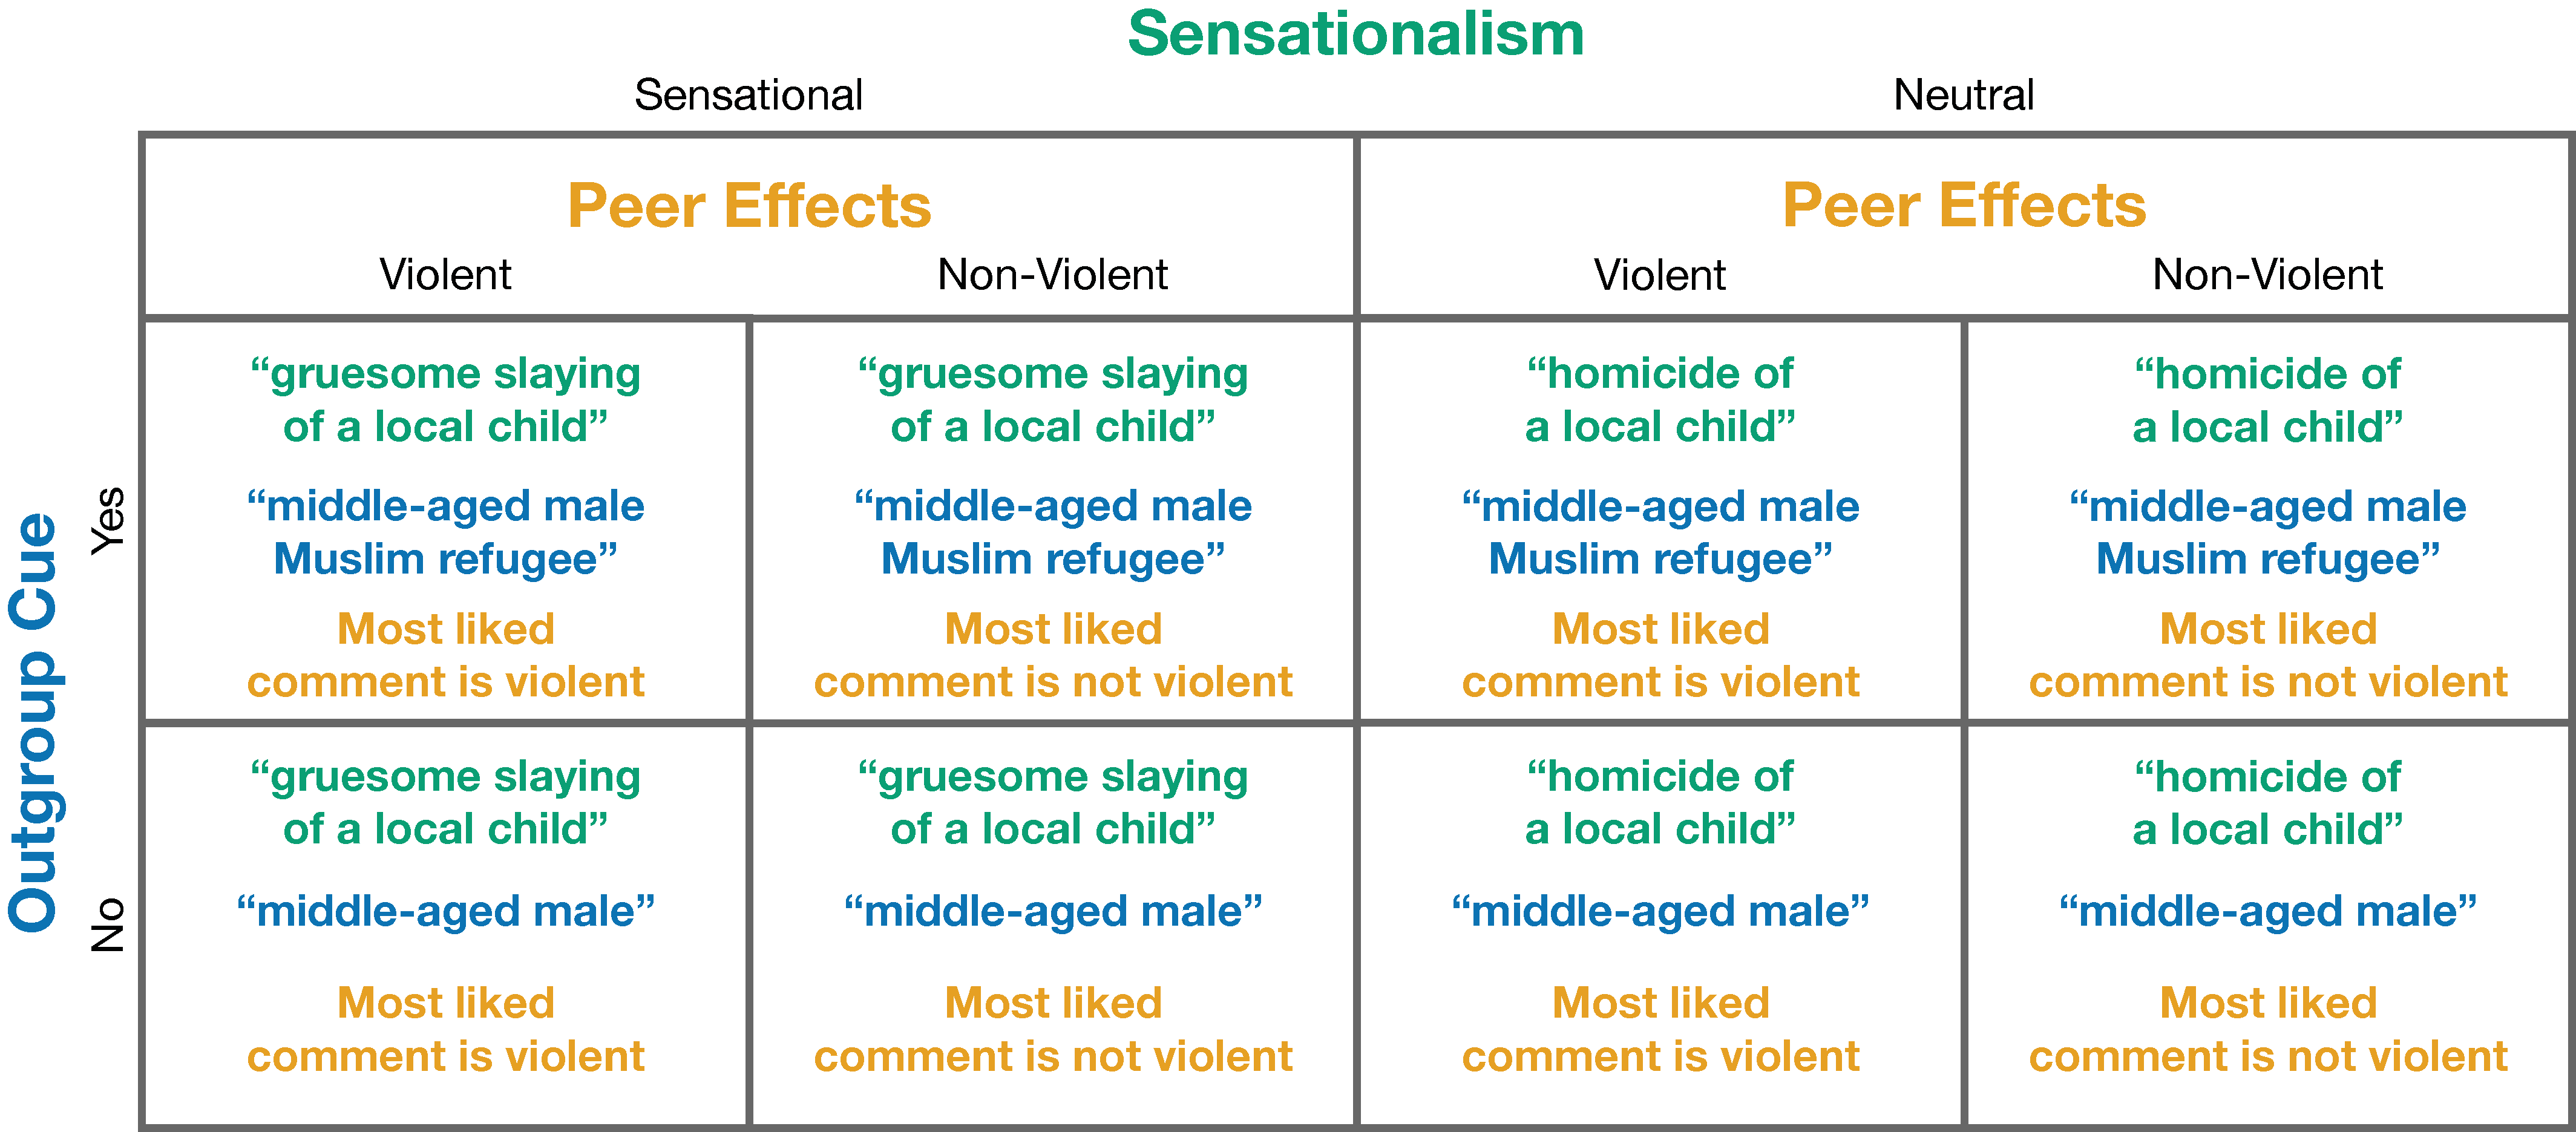
\includegraphics[width=\textwidth]{figures/treatment_table.pdf}
    \begin{minipage}{\textwidth}
      \footnotesize
      \setlength{\parskip}{0pt}
      \setlength{\parindent}{0pt}
      For the \textcolor{colorSensationalism}{``sensationalism''} treatment, the title for neutral group includes ``homicide of a local child'' (1-4) and the sensational group title includes ``gruesome slaying of a local child'' (5-8). For the \textcolor{colorOutgroupCue}{``outgroup cue''} treatment, the non-Muslim group sees the alleged perpetrator described as a ``middle-aged male'' (1,2,5,6) and the Muslim group sees him described as a ``middle-aged male Muslim refugee'' (3,4,7,8). For the \textcolor{colorPeerEffects}{``peer effects''} treatment, for the non-violent group, the most liked comment is non-violent (1,3,5,7), and for the violent group the most liked comment is violent (2,4,6,8).
    \end{minipage}
\end{figure}


The pre-treatment survey contained a battery of background questions concerning respondents' demographic characteristics, party identification, and individual dispositions towards authoritarianism, symbolic racism, and ethnocentrism. We use \cite{feldman1997perceived}'s four-item Child Rearing Values (CRV) scale to measure authoritarian personality. Our symbolic racism and ethnocentrism scales are taken directly from ANES. We calculate ethnocentrism by averaging outgroup feeling thermometers towards Asians, Blacks, Hispanics, Muslims, and refugees. We calculate symbolic racism by averaging the four items from the ANES symbolic racism scale, reversing two items to make the scale range from low to high racism.

The post-treatment survey asked a series of questions regarding respondents' emotional responses to the homicide and the attack on the alleged perpetrator, separately. These emotion questions were measured to test the outrage-punitiveness hypothesis. Each emotion barometer asks respondents to indicate their felt intensity of eight emotions using five-point scales. To avoid biasing respondents' emotional reactions, we included a list of eight emotions, positive and negative, based loosely on Robert Plutchik's typology of basic discrete emotions.

We measured violent attitudes, directly and indirectly, using survey scale and open-ended responses. To measure punitiveness toward the alleged perpetrator in the story, we asked respondents to rate their support for nine punishments on seven-point (-3 to 3) scales. To test for support for extrajudicial violence, we ask if the perpetrator should be tortured and if he should be jailed without trial. Because direct questions about violence are subject to social desirability bias, we included indirect measures of punitiveness. We asked respondents how they think the locals who engaged in street violence against the suspect should be punished for beating the homicide suspect, and we ask if they would be willing to donate to a legal defense fund for the attackers. To measure punitiveness toward outgroups, we presented respondents with four seven-point (-3 to 3) scales to indicate their support for or opposition to policies on refugee immigration, Muslim immigration, and monitoring and registering Muslim communities.

In addition to these survey scale responses, we collected behavioral data on respondents' interaction with the news website and text data from respondents' written reactions to the article. Our survey instructions encouraged respondents both to read the article and to interact with the website by liking, reporting, or posting comments in the comments section below the text of the news story, though doing so was not mandatory. Respondents' comments and any clicks on ``report'' or ``like'' buttons were stored in our database as behavioral measures of support or disapproval of violence. We asked respondents to provide twenty-word responses to the homicide and the mob attack on the suspect in two separate open-ended questions. We devised a novel typology to classify violent content (see Figure S16, p. 23), which a team of four researchers, blind to treatment condition, used to hand annotate all text data collected in open-ended responses and comments. Coding rules were pre-registered\footnote{See preregistration on EGAP here: http://egap.org/registration/5345.} before our survey and involved categories (and subcategories) such as violence (lethal violence, extrajudicial violence, judicial violence, forcible physical displacement, property destruction/confiscation), group mentions (ingroup mention, race, religion, etc.), and attacks (dehumanizing, demonizing). We detailed these coding rules in flow-charts that were used in weekly training sessions and as a reference for coders. Agreement between coders was nearly perfect according to Cohen's kappa and Krippendorf's alpha and F1 measures (see Table S14, p. 24).\footnote{To measure inter-coder reliability, two coders coded a random sample of open-ended responses. Cohen's kappa and Krippendorf's alpha are inter-coder reliability measure for nominal scales and two coders. Though there is no agreed-upon interpretation of the kappa coefficient, it has been  suggested  that 0.61-0.80 indicates substantial  agreement, and 0.81-1.0 indicates near-perfect agreement. F1 is a common performance measure in machine learning ranging from 0 to 1. It is defined as the harmonic mean of precision and recall. F1 is a good measure of coder agreement when choices are imbalanced. With imbalance in choices, percent agreement (accuracy) will overestimate coder agreement.} Though the University of Michigan IRB reviewed this study and deemed it exempt, we went to great lengths to ensure that our experimental treatment did not cause harm. To ensure that the study did not cause harm to respondents or others, we debriefed respondents to ensure that they understood that the news article we presented was fictitious and why the study required this use of deception. This was done in bold text with very clear language and required the respondent to acknowledge the statement. The research design, text coding scheme, and the experimental vignettes for this study were pre-registered before conducting the study.

Our sample of 1655 respondents, recruited through Amazon's Mechanical Turk (MTurk) in early December 2018. To mitigate potential problems arising from automation and lack of demographic representativeness in MTurk samples, we collected extra metadata from respondents to identify bots, and purposively oversampled women, baby boomers, non-whites, and Republicans using Turk Prime. Despite our concerns with MTurk, many recent studies have suggested that MTurk samples can in fact be more reliable than traditional survey pools.\footnote{Recent work has found MTurk workers more reliable than subject pool workers in their level of attention \citep{white_strezhnev_lucas_kruszewska_huff_2018} and when it comes to the issue of researcher demand \citep{Hauser2016}.} We screened according to predicted bots {\it and} failed attention checks. Our resulting sample roughly approximated the demographics of the American population. Within our sample, 49 percent identified as female and 77 percent as white, in line with the US Census Bureau's 2018 population estimates of 51 percent and 77 percent, respectively. The median age of our respondents was 36, versus 38 in the population. Looking at Gallup's 2017 estimates of party affiliation, our sample was over-represented in self-identified Democrats (41.3 percent versus 29 percent) but proportionally representative of Republicans (28 percent). To ensure proportional geographic representativeness, we stratified our sampling according to the population size of each of the nine regional divisions designated by the US Census Bureau. This sample includes non-compliers who failed an attention check and respondents who received the treatment but did not finish the survey. Both noncompliance and attrition were extremely low: less than 1 percent failed the attention check, and 2.54 percent did not complete the entire post-treatment survey. It is clear from the open-ended questions that respondents were attentive to the treatments. We ran a $\chi^2$ test of independence across term counts in each treatment group and found that key words mapped onto the content and sentiment of the treatments (see Figures S11-S13, pp. 13-14). Here we conduct an intent-to-treat analysis and do not exclude subjects on any post-treatment variables. The supplementary material (pp. 1-5) provides an in-depth description of the sampling and randomization process.

\section{Results}

\begin{comment}
    - "It is unclear why social desirability bias leads to null results in this setting (it is usually the opposite in these cases since the treatment is strong and straightforward). Can the authors expand on this? Also, was this choice pre-registered? If not, the authors are reporting only the results that converge to their hypotheses. I would discourage this, and ask authors to report the full set of results."
    - "the data does not support the first hypothesis of the article. Effects are only detected for one outcome, out of ten! ...the authors should report null results, and explain why their open-text measures are positive (which, in my view, might have something to do with social desirability bias)."
    - Should add short text descriptions to EVERY figure in the text. "The behavioral outcomes in Figure 4 are the most interesting and are also the ones that are most important for the social media literature. I did not understand the results from Figure 5."
    - "My biggest quibble with the authors is how they present the data. I think that can be greatly improved. The authors have 8 treatment conditions, and I was expecting a presentation of the average treatment effects across each condition."
\end{comment}

\subsection{Sensational Content Hypothesis}

\vspace{1em}
\noindent\textbf{Sensational content hypothesis:} content that sensationalizes moral transgressions increases tolerance or support for violence (punitiveness).
\vspace{1em}

As expected for the sensational content hypothesis, the sensational content treatment significantly increased support for violence when measured indirectly through questions about the mob attack on the alleged perpetrator and open-ended responses on the events in the article. However, we did not find significant average treatment effects for sensational content on punitiveness when looking at survey scale questions that directly asked respondents what kinds of punishments they would support for the alleged perpetrator in the article (see Figure S7, p. 6). We expected these direct measures to be vulnerable to social desirability bias due to the presence of very extreme violence at the end of some of these scales (e.g., ``public execution via firing squad,'' and torture). It's worth noting that the one significant level of this scale is indefinite detention, which according to qualitative readings of open-ended responses, appeared to be a palatable punishment that was also not seen as too lenient. Respondents presented with sensational content were more likely to donate to a legal defense fund for people who engaged in a mob attack on the alleged perpetrator (\textit{P} $<$ 0.05), and were more likely to believe that not punishing them was justified. However, this finding is not statistically different from zero at conventional levels of significance (Figure 2), and thus serve as merely suggestive evidence. This effect for sensational content further holds when looking at the text data from the open-ended responses. We find that sensational content significantly increased the probability that respondents will express support for violence in their written responses, including extrajudicial, mob-style violence (\textit{P} $<$ 0.05); for both measures this effect represents a roughly fifteen percent increase in probability (Figure 3). Note that the survey scale and text measures of support were highly correlated. Expression of support for violence in the open-ended responses significantly and positively correlates with indirect survey scale responses as well as support for the death penalty for the alleged perpetrator (all \textit{P} $<$ 0.001) (see Figure S6 and Table S1, p. 5-6).

A cursory comparison of representative open-ended responses illustrate differences in punitiveness across treatment conditions. One respondent given the sensationalized content treatment wrote the following, which was coded as supportive of violence: ``I am absolutely disgusted, appalled, and at a loss for words about this attack.  They should kill him in the street. Let everyone who wants a piece of him have a piece of him.'' Contrast this with a non-violent response in the control condition: ``I want to know what happened. I want to know if the person that was beat up is the one accused of the murder. I want to know the details.'' See the supplementary material (pp. 16-17) for representative open-ended responses and comments by coding category and treatment condition.

\begin{figure}[!htbp]
  \centering
  \caption{Support for the Mob Attack by Treatment Condition}
  \includegraphics[width=.835\textwidth]{figures/ATE_punish_mob_outcomes.pdf}
\end{figure}

\begin{figure}[!htbp]
  \centering
  \caption{Support for Violence in the Open-ended Responses by Treatment Condition}
  \includegraphics[width=.835\textwidth]{figures/ATE_oe.pdf}
\end{figure}

\subsection{Outgroup Cue Hypothesis}

\vspace{1em}
\noindent\textbf{Outgroup cue hypothesis:}  content that sensationalizes the moral transgressions of a member of a particular outgroup will increase negative attitudes toward that outgroup.
\vspace{1em}

Unexpectedly, outgroup cues decreased support for violence against the perpetrator in the story when measured indirectly and in the open-ended responses (\textit{P} $<$ 0.05) and do not support the outgroup cue hypothesis (Figures 1 and 2). That being said, we do suspect this negative effect was driven by perceptions that the event or even the article itself were colored by racial bias or animus. Respondents explicitly moderated their responses to cater toward a socially desirable standard and were significantly more likely to believe that the mob attack or the article itself was racially-motivated when given the outgroup treatment (see Figures S14-15, p. 22).

Our results support the bandwagoning hypothesis and shed light on how sensational content and violent peer influence affect interactions with online content. The sensational content treatment increased the probability that respondents would leave a comment on the website by roughly sixteen percent (\textit{P} $<$ 0.05) (Figure 4). Since the act of leaving a comment is vulnerable to significant selection effects, we run Heckman two-step selection models to detect and correct for selection bias \citep{heckman1979sample}. Older respondents and respondents scoring high on symbolic racism were far more likely to leave a comment. After taking this into account, we find that the sensational treatment increased the probability of writing a violent comment by roughly twenty-four percent, though this effect is not statistically significant at conventional levels (\textit{P} $=$ 0.14 level) (Figure 5).\footnote{We include effects that are not statistically significant because they offer suggestive evidence of our theory.}

\subsection{Bandwagoning Hypothesis}

\vspace{1em}
\noindent\textbf{Bandwagoning hypothesis:} individuals will be more likely to ``like'' or leave a comment that supports the use of violence (judicial or extrajudicial) if they perceive that a pro-violence stance is the majority position.
\vspace{1em}

While peer signals mattered little for attitudinal outcomes, they consistently affected how respondents interacted with the news article, creating a ``cascade effect'' \citep{bikhchandani1992theory} for endorsement of violence. That is, respondents bandwagoned onto violent comments if they were already highly-liked. If the top, most-liked comment was violent, respondents were more likely to like a violent comment (\textit{P} $<$ 0.05) and to leave a violent comment of their own (\textit{P} $<$ 0.05); and far less likely to like a non-violent comment (\textit{P} $<$ 0.001) (Figures 3 and 4). Also, respondents were less likely to report the violent comment when it was highly liked, though this effect was not statistically significant (\textit{P} $=$ 0.12). Because the most liked comment was also positioned at the top of the three comments---as is usually the case in a comments section on a news website---this effect may possibly be driven by the position of the comment rather than the fact that it was highly liked; that is, respondents may have been merely satisficing by interacting with the upvoted violent comment because it was at the top of comment list. We believe the violent comment's upvoting was more important than its positioning for two reasons. First, we found that the upvoted violent comment treatment had a \textit{negative} effect on reporting the violent comment and a \textit{positive} treatment effect on expressing violence in a written comment, which suggests the effect is not due to merely interacting with whatever comment was positioned at the top of the comments list. Second, each comment was only one or two lines long, so users would have seen all three comments at once when they scrolled down; it is unlikely that the bottom two comments would have been less visible to respondents.

\begin{figure}[!htbp]
  \centering
  \caption{Behavioral Outcomes by Treatment Condition}
  \includegraphics[width=.835\textwidth]{figures/ATE_behavioral.pdf}
\end{figure}


\begin{figure}[!htbp]
  \centering
  \caption{Comment Outcomes by Treatment Condition}
  \includegraphics[width=.835\textwidth]{figures/ATE_com_heckman.pdf}
\end{figure}

\subsection{Outrage-Punitiveness Hypothesis}

\vspace{1em}
\noindent\textbf{Outrage-punitiveness hypothesis:} Outrage is the emotional mechanism through which content containing sensationalized moral transgressions increases support for violence. As such, sensationalized moral transgressions are more likely to elicit stronger feelings of outrage from respondents, and respondents who feel more outraged will be more supportive of harsher punishment of or violence against the perceived transgressor.
\vspace{1em}

In line with the outrage-punitiveness hypothesis, sensational content elicited strong emotional responses of anger (\textit{P} $<$ 0.1), fear (\textit{P} $<$ 0.05), and anxiety (\textit{P} $<$ 0.05) from respondents, while outgroup cues and peer support did not (Figure 6). To gauge whether emotional mechanisms mediated the treatment effect of sensational content on violent attitudes and behavior, we use causal mediation analysis \citep{imai2011commentary}. Because emotion was not randomly assigned, violating the assumption of sequential ignorability, we include possible confounding covariates to the models---i.e., measures of authoritarianism \citep{stenner2005authoritarian}, ethnocentrism \citep{kinder2010us}, symbolic racism \citep{banks2014anger}, and whether the respondent resided in the American South \citep{nisbett1996culture}. Causal mediation analysis revealed that anger, fear, and anxiety mediated the effect of sensational content on support for the mob attackers' legal defense fund (\textit{ACME} = 0.06, 0.04, and 0.03, respectively; all \textit{P} $<$ 0.05) and the likelihood of expressing support for violence in the open-ended responses (\textit{ACME} = 0.007, 0.003, and 0.002, respectively; all \textit{P} $<$ 0.1) (see Figures S8-10, pp. 12-13). We do not find emotional mediating effects for the other two treatments or behavioral and anti-outgroup outcomes.

\begin{figure}[!htbp]
  \centering
  \caption{Emotional Response by Treatment Condition}
  \includegraphics[width=.835\textwidth]{figures/ATE_emotion.pdf}
\end{figure}

Did this increased punitiveness translate into support for sanctions on Muslims and refugees? We find sensational content and peer support for violence did not increase support for anti-Muslim and anti-refugee policies; however, the mere inclusion of an outgroup cue on average increased support for anti-Muslim and anti-refugee policies (Figure 7). Identifying the alleged perpetrator as a Muslim refugee caused respondents to support tightening refugee quotas (\textit{P} $<$ 0.1) and restricting Muslim immigration  (\textit{P} $<$ 0.05), and positive for support for increased monitoring of Muslims  (\textit{P} $<$ 0.05) and approval of a Muslim ``registry'' (\textit{P} $<$ 0.1). This finding contrasts with the earlier finding that including an outgroup cue increased individuals' suspicion that the attack described in the article, or the article itself, was racist. Indeed, this contradiction appeared in some of the open-ended responses in the outgroup cue treatment condition. One respondent in the outgroup cue treatment condition wrote: ``I was thinking it was a fake story to invoke Islamophobia...I also do not want them moving next door to me or in our country, they can keep their backwards traditions in their own countries.'' Perceived racial bias or untrustworthiness of the content's source did not temper respondents' attitudes towards Muslims and refugees.

\begin{figure}[!htbp]
  \centering
  \caption{Support for Anti-Muslim Policies by Treatment Condition}
  \includegraphics[width=.835\textwidth]{figures/ATE_punitive.pdf}
\end{figure}

This increased punitiveness towards refugees and Muslims may be a function of a general increase in punitiveness. Outrage arising from morally transgressive behavior may trigger an ``intuitive prosecutor'' mindset that heightens one's desire to punish all subsequent transgressors, regardless of their connection to the original transgressor \citep{crockett2017moral, goldberg1999rage, tetlock2007}. To this end, we looked at the effects of the treatments on preferences regarding punishment of homicide, the crime featured in the article. We did not find a significant effect between sensational content, outgroup cues, or peer support on respondents' attitudes towards the punishment of homicide. 

Contrary to our expectations, we did not find a significant interaction effect between outgroup cues and moral-emotional content on anti-immigrant and anti-Muslim policy preferences, and the effect is not in the expected direction. The average treatment effect for peer support is insignificant, as is its interaction between outgroup cues, though the signs of these effects are in their expected direction (see Table S5, p. 10). In the open-ended text outcomes, our outgroup cue triggered explicit remarks about social-desirability and discussions of racism (see Figure S14, p. 22). In addition to qualitative examination of these comments, it is clear that respondents were hesitant to be support violence out of concerns that racism played into the behavior of those involved.  We believe the effect of outgroup cues on punitiveness and support for violence merit further study with a more subtle treatment.

\section{Discussion}

\begin{comment}
    - "The unexpected outgroup cue effect is awkward. It sounds like greater design care is needed in future studies to directly test whether socially desirable responding really was the explanation. It might be worth outlining what such a test might look like in the discussion."
\end{comment}

This study contributes to our understanding of sensational news and mass opinion in three ways. First, this is one of the first studies, to our knowledge, to demonstrate the causal effects of rage bait consumption on attitudes towards violence and online behavior. Second, it situates rage bait in the larger conceptual field of misinformation. Third, it identifies the importance of both anger and fear as emotional mediators of the effects of rage bait on punitiveness. Fourth, we show that the threshold by which content increases anti-outgroup sentiment is rather low: simply attributing a crime to a member of a certain outgroup is sufficient to increase discriminatory attitudes. Contrary to research that explicit outgroup cues do not increase support for anti-outgroup policies \citep{huber2006race,mendelberg2001race} or are unnecessary \citep{banks2016group}, we find that outgroup cues increase punitiveness towards an outgroup even when these cues raise concerns about racial bias.

One key limitation of our study is a lack of statistical power stemming from the authors' resource constraints. This limited the size of each treatment block, resulting in a handful of effects that were outside conventional levels of statistical significance.

Understanding the importance of online content in political life has perhaps never been more critical than in the present. While these findings are a far cry from evidence that sensational news mobilizes on-the-ground violence, they underscore the importance of content and discourse in inflaming violent attitudes and carry significant policy implications for governments and social media companies working to stem the harmful effects of sensational news, especially sensationalized false news. 

While outside the scope of this study, we believe that these findings are not restricted to the contemporary false news phenomenon or even online content: the use of sensational content to mobilize violence has a long genealogy. Why leaders choose these strategies for mobilizing popular support for violence and when they translate into on-the-ground violence remain crucial and promising areas for future scholarly inquiry.

Finally, while anti-Muslim sentiment manifests in similar ways to other outgroups (e.g., strong correlations with ethnocentrism, authoritarianism, etc.), it is also distinct. Anti-Muslim sentiment is driven by both cultural {\it and} racial/religious minority affect while other minority outgroups are driven by one or the other \citep{doi:10.1017/S0022381609090756}. As such, this study is limited in scope to the particular case of Muslim Americans.

%\section{Acknowledgments}
%We would like to thank the Lieberthal-Rogel Center for Chinese Studies and the Rackham Graduate School at the University of Michigan for their generous funding. We would also like to thank our research assistants, Grace Phillips and Lyla Yu, for their help with text annotation. We would also like to thank Pablo Barbera, Iza Ding, Mary Gallagher, Mai Hassan, Hakeem Jefferson, Tom O’Mealia, Walter Mebane, Steven Moore, Dan Slater, Mike Thompson-Brusstar, Nick Valentino, Nicole Wu, and members of the Center for Political Studies Workshop and the Comparative Politics Workshop at the University of Michigan for their feedback on previous drafts of this paper.

%\section{Competing Interests}
%The authors declare no competing interests.

% BJPOLS uses footnotes, not endnotes. \endnote in this template will behave like \footnote; and \printendnotes will not output anything.
% \printendnotes

\printbibliography

\appendix

%\input{sources.bib}

\end{document}
